\documentclass[12pt, a4paper]{article}
\usepackage{../../../../../style}
\begin{document}
	\lhead{Группа 91} \chead{Модуль 6 Занятие №3} \rhead{Школа <<Симметрия>>}
	\begin{wrapfigure}{r}{0.5\textwidth}
		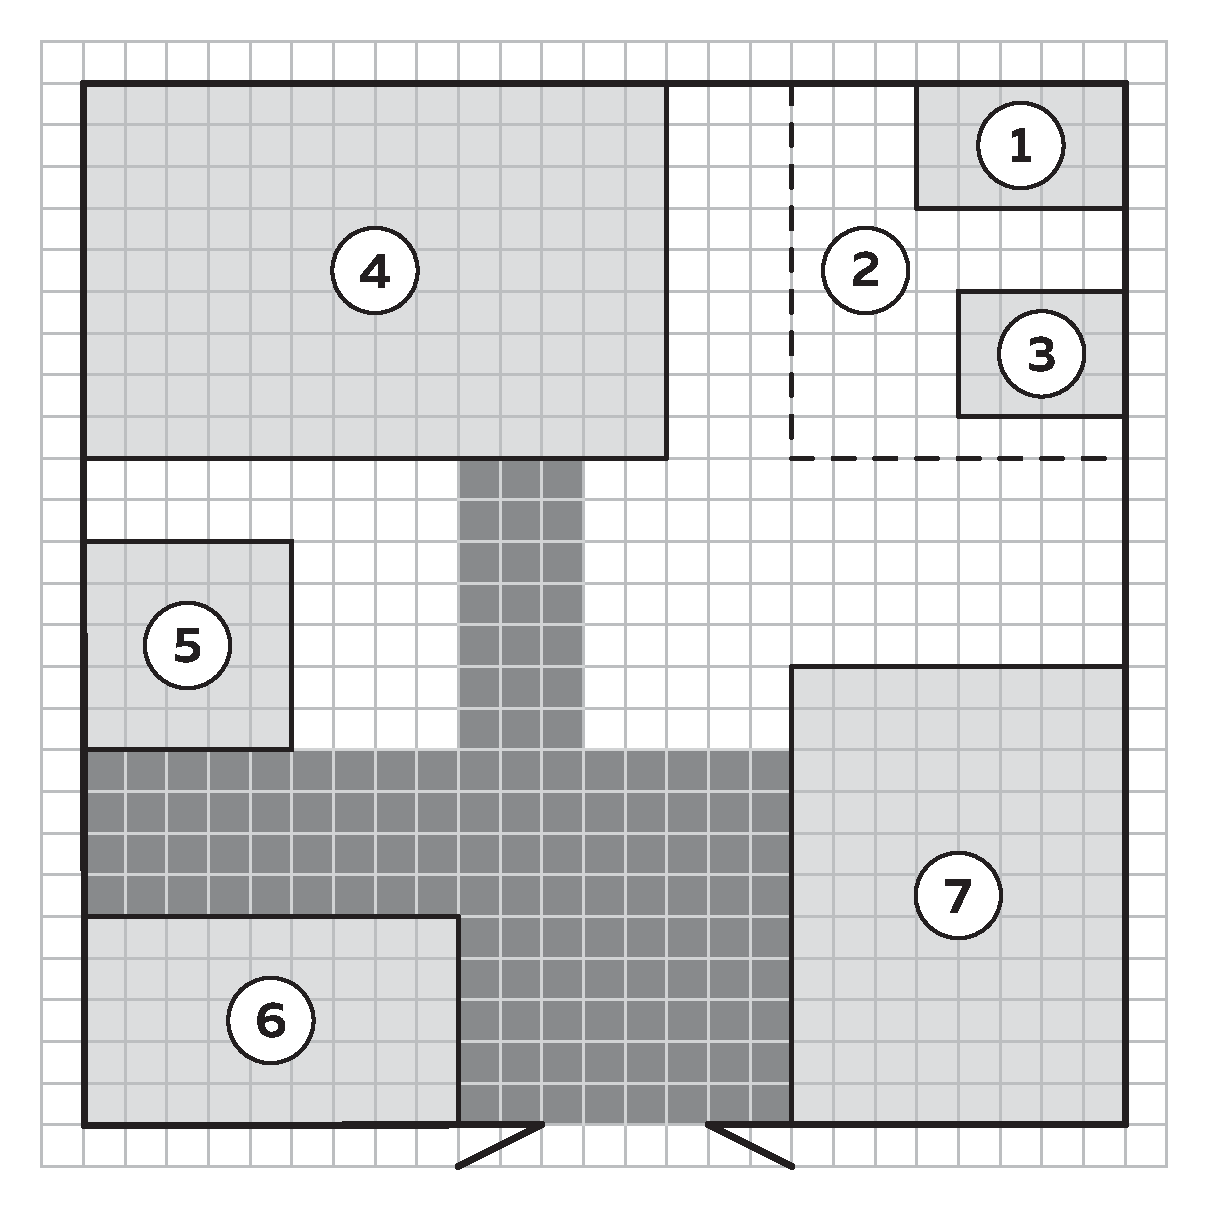
\includegraphics[width=0.5\textwidth]{plan}
	\end{wrapfigure}
	На плане изображено домохозяйство (сторона каждой клетки на плане равна $0,5$ м). Участок имеет квадратную форму.
	
	При входе на участок справа от ворот находится гараж на два машиноместа, а слева — летний домик, отмеченный на плане цифрой 6. Площадь, занятая летним домиком, равна $11,25$ м$^2$.
	
	Жилой двухэтажный дом находится в глубине территории. Оба этажа имеют одинаковую площадь. Помимо летнего домика, жилого дома и гаража, на участке имеется баня, расположенная неподалеку от летнего домика, и теплица, построенная на территории огорода (огород отмечен цифрой $2$). Также в углу огорода расположена компостная яма.
	
	Все дорожки внутри участка вымощены тротуарной плиткой размером $0,5$ м × $0,5$ м. Между гаражом и летним домиком, а также между летним домиком и баней имеются площадки, вымощенные такой же плиткой. К домохозяйству подведено электричество. Имеется магистральное газоснабжение.
	
	\begin{enumerate}
		\item Для объектов, указанных в таблице, определите, какими цифрами они обозначены на схеме. Заполните таблицу, в ответ запишите последовательность четырёх цифр.
		\begin{table}[!h]
			%
			\renewcommand{\arraystretch}{1.4} % larger cell height
			\centering
			%
			\begin{tabular}{|c|c|c|c|c|}
				\tend
				Объекты & Гараж & Летний домик & Баня & Жилой дом \\
				\tend
				%
				\thead Цифры & & & & \\
				\tend
			\end{tabular}
		\end{table}
		\item Найдите площадь обоих этажей жилого дома (в м$^2$).
		\item Хозяин участка планирует вырыть перед домом колодец диаметром $3$ м. Найдите площадь, которую будет занимать этот колодец. Ответ дайте в виде $\dfrac{S}{\pi}$.
		\item На сколько процентов площадь гаража больше площади летнего домика?
		\item Найдите периметр забора вокруг участка.
		\item Найдите расстояние между противоположными углами теплицы.
		\item Вычислите:
		\begin{multicols}{2}
			\begin{enumerate}[label=\asbuk*)]
				\item $48\cdot(0,6\cdot5-2,875)\cdot0,25$
				\item $4\dfrac{2}{21}\cdot10-19\dfrac{20}{21}$
				\item $\left(\dfrac{2}{15}+1\dfrac{7}{12}\right)\cdot\dfrac{30}{103}-\left(2:2\dfrac{1}{4}\right)\cdot\dfrac{9}{32}$
			\end{enumerate}
		\end{multicols}
	\newpage
		\item \subimport{../../../../../exercises/arithmetic/coordinate_line/fractions}{ex_2}
		\item \subimport{../../../../../exercises/arithmetic/coordinate_line/roots}{ex_2_1}
		\item Найдите значение выражения $\dfrac{\sqrt{300}\cdot\sqrt{72}}{2\sqrt{3}}$\\
		\textit{В ответе укажите номер правильного варианта.}
		\begin{multicols}{4}
			\begin{enumerate}[label=\arabic*)]
				\item $10\sqrt{5}$
				\item $20\sqrt{3}$
				\item $30\sqrt{2}$
				\item $15\sqrt{3}$
			\end{enumerate}
		\end{multicols}
		\item Решите уравнения:
		\begin{multicols}{2}
			\begin{enumerate}[label=\arabic*)]
				\item $3x(2x-7)=0$
				\item $2x^2-3,1x+0,42=0$
			\end{enumerate}
		\end{multicols}
		\item В коробке $14$ пакетиков с чёрным чаем и $6$ пакетиков с зелёным чаем. Павел наугад вынимает один пакетик. Какова вероятность того, что это пакетик с зелёным чаем?
		\item Расстояние $S$ (в метрах) до места удара молнии можно приближенно вычислить по формуле $S=330\cdot t$, где $t$ --- количество секунд, прошедших между вспышкой молнии и ударом грома. Определите, на каком расстоянии от места удара молнии находился наблюдатель, если гром он услышал через $10$ секунд после вспышки. Ответ дайте в километрах.
		\item Решите неравенство $-3-x>4x+7$.\\ \textit{В ответе укажите номер правильного варианта.}
		\begin{multicols}{2}
			\begin{enumerate}[label=\arabic*)]
				\item $(-\infty;-0,8)$
				\item $(-2;+\infty)$
				\item $(-0,8;+\infty)$
				\item $(-\infty;-2)$
			\end{enumerate}
		\end{multicols}
		\item Решите уравнения:
		\begin{multicols}{2}
			\begin{enumerate}[label=\asbuk*)]
			\item $x^4+2x^2-3=0$
			\item $3x^3-7x^2-7x+3=0$
			\end{enumerate}
		\end{multicols}
	\end{enumerate}
\end{document}